

\section{Supplemental Figures}
\label{paperB:supp:supplemental_figures}

\begin{figure}[ht!]
    \centering
    \begin{minipage}{0.95\textwidth}
        \centering
        \begin{subfigure}[t]{0.82\linewidth}
        	\centering
        	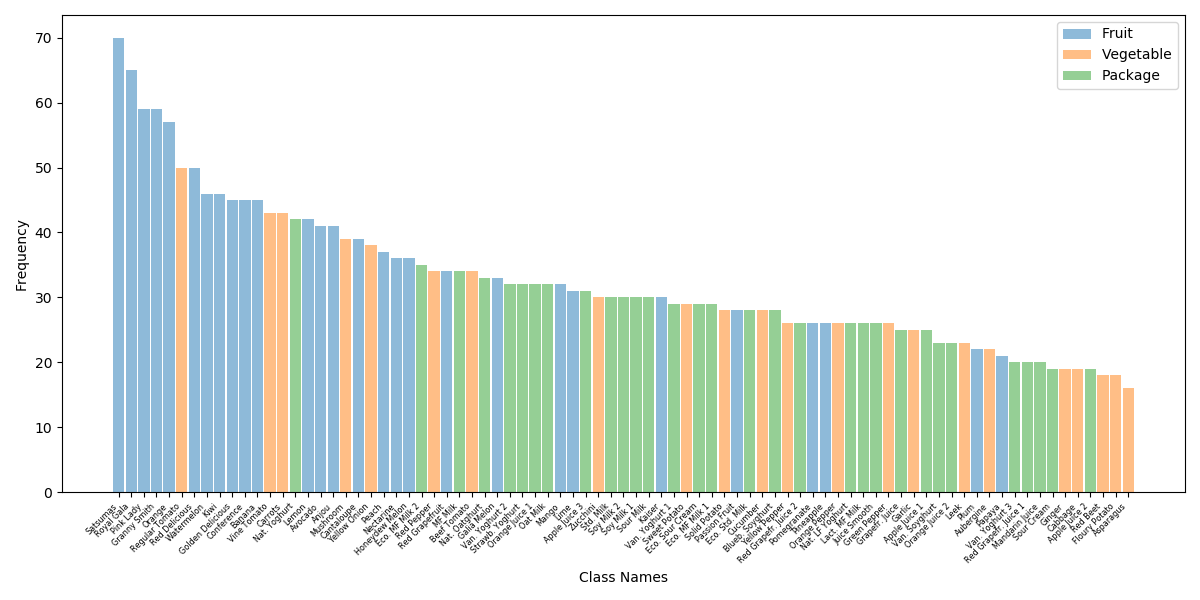
\includegraphics[width=\textwidth]{PaperB/appendix/figures/class_distributions_histogram/class_dist_train.png}
        	%\vspace{-7mm}
        	\caption{Histogram for the training split.}
        	\label{fig:class_distribution_train}
        \end{subfigure} \\
        \begin{subfigure}[t]{0.82\linewidth}
			\centering
			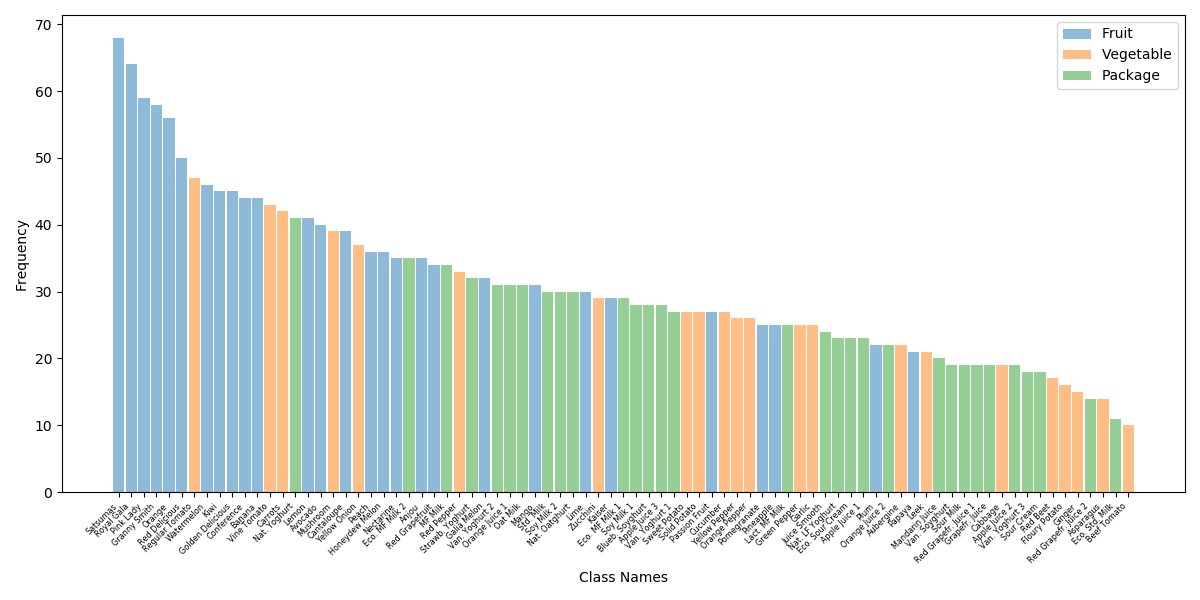
\includegraphics[width=\textwidth]{PaperB/appendix/figures/class_distributions_histogram/class_dist_test.png}
			%\vspace{-7mm}
			\caption{Histogram for the test split.}
			\label{fig:class_distribution_test}
		\end{subfigure} \\
        \begin{subfigure}[t]{0.82\linewidth}
			\centering
			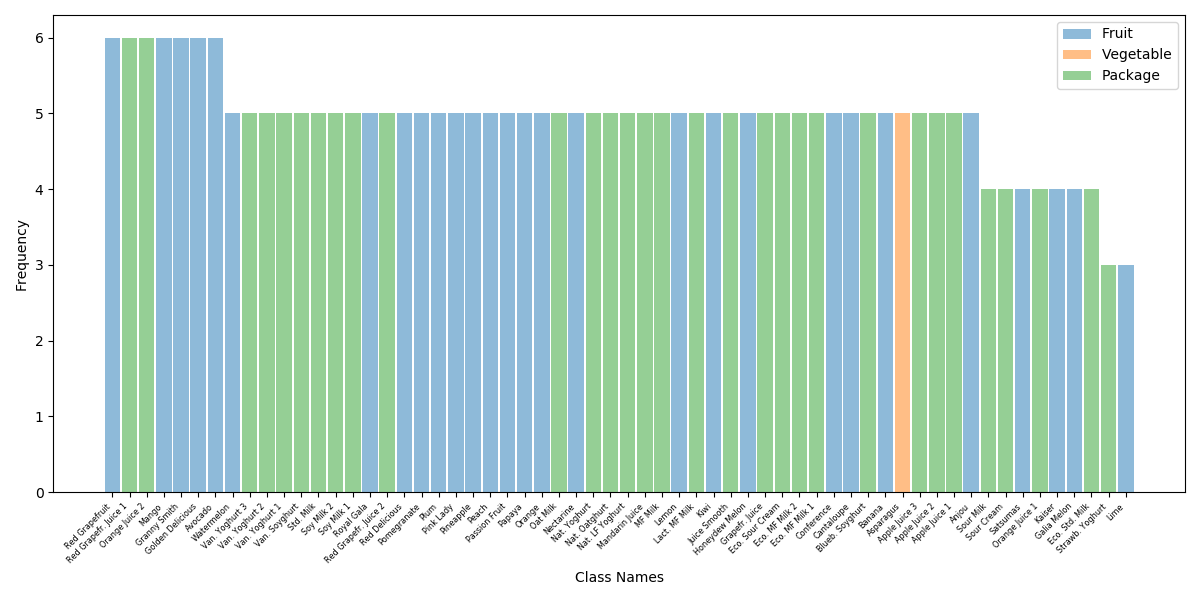
\includegraphics[width=\textwidth]{PaperB/appendix/figures/class_distributions_histogram/class_dist_val.png}
			%\vspace{-7mm}
			\caption{Histogram for the validation split.}
			\label{fig:class_distribution_val}
		\end{subfigure} 
    \end{minipage}
    \caption{Histograms of natural images for every class in the training (a), test (b), and validation (c) splits of the Grocery Store dataset. We also show with different colors on the bins if the class is either a Fruit, Vegetable, or Package item.}
    \label{fig:histograms}
\end{figure}
\clearpage
%\pagebreak

\begin{figure}[t] 
\centering
\begin{subfigure}[t]{0.48\textwidth}
	\centering
	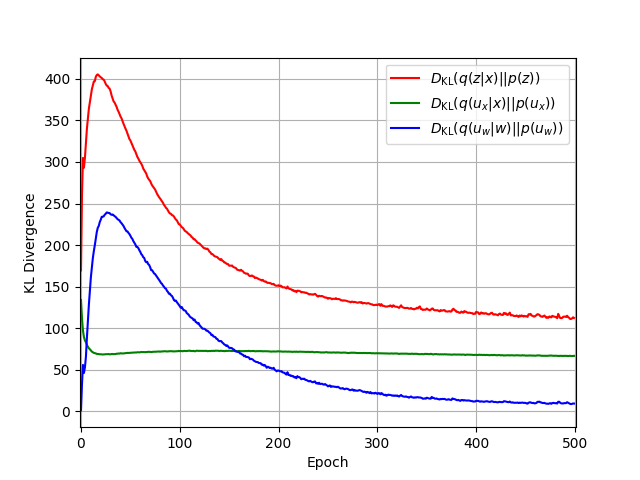
\includegraphics[width=\textwidth]{PaperB/appendix/figures/kl_divergence/kl_vcca_private_xw.png}
	\caption{VCCA-private$_{x w}$}
	\label{subfig:kl_divergence_vcca_private_xw}
\end{subfigure}~
\begin{subfigure}[t]{0.48\textwidth}
	\centering
	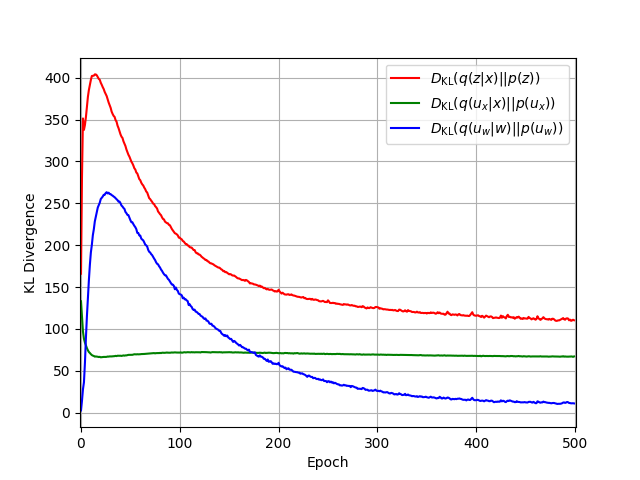
\includegraphics[width=\textwidth]{PaperB/appendix/figures/kl_divergence/kl_vcca_private_xwy.png}
	\caption{VCCA-private$_{x w y}$}
	\label{subfig:kl_divergence_vcca_private_xwy}
\end{subfigure}
\caption{The measured KL divergences $\KL(q_{\phi_{z}}(z|x)\,||\,p(z))$ (red), $\KL(q_{\phi_{x}}(u_{x}|x)\,||\,p(u_{x}))$ (green), and $\KL(q_{\phi_{w}}(u_{w} |w)\,||\,p(u_{w}))$ (blue) over epochs. We increased the number of epochs from 200 to 500 to demonstrate that the KL divergence for the private latent variable $u_{w}$ goes to zero. The number of words $T=24$ is the same for both models. The likelihood weights are set to $\lambda_{w} = 1000$ and $\lambda_{y} = 100$. Abbreviations: VCCA, Variational Canonical Correlation Analysis; KL, Kullback-Leibler.
}
\label{fig:kl_divergence_vcca_private}
\end{figure}

\begin{figure}[t] 
\centering
\begin{subfigure}[t]{0.48\textwidth}
	\centering
	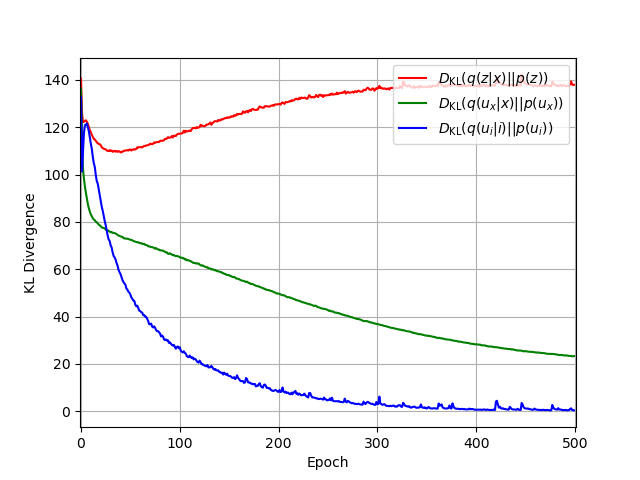
\includegraphics[width=\textwidth]{PaperB/appendix/figures/kl_divergence/kl_div_vcca_private_xi.png}
	\caption{VCCA-private$_{x i}$}
	\label{subfig:kl_divergence_vcca_private_xi}
\end{subfigure}~
\begin{subfigure}[t]{0.48\textwidth}
	\centering
	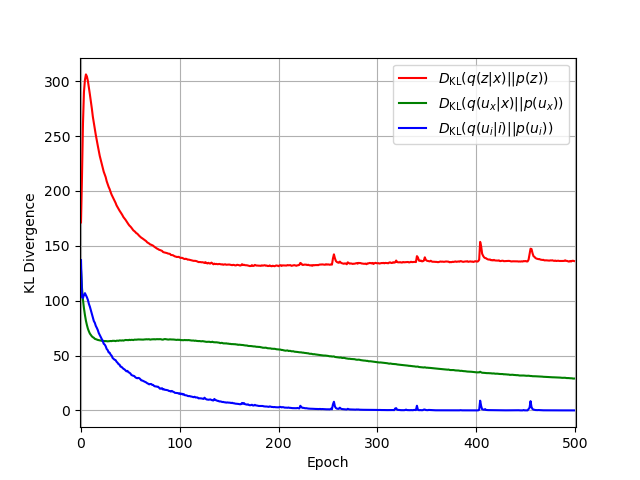
\includegraphics[width=\textwidth]{PaperB/appendix/figures/kl_divergence/kl_div_vcca_private_xiy.png}
	\caption{VCCA-private$_{x i y}$}
	\label{subfig:kl_divergence_vcca_private_xiy}
\end{subfigure}
\caption{The measured KL divergences $\KL(q_{\phi_{z}}(z|x)\,||\,p(z))$ (red), $\KL(q_{\phi_{x}}(u_{x}|x)\,||\,p(u_{x}))$ (green), and $\KL(q_{\phi_{i}}(u_{i} |i)\,||\,p(u_{i}))$ (blue) over epochs. We increased the number of epochs from 200 to 500 to demonstrate that the KL divergence for the private latent variable $u_{i}$ goes to zero. The likelihood weights are set to $\lambda_{i} = 10$ and $\lambda_{y} = 1000$. Abbreviations: VCCA, Variational Canonical Correlation Analysis; KL, Kullback-Leibler. 
}
\label{fig:kl_divergence_vcca_private_with_iconic_image}
\end{figure}


\clearpage
%\pagebreak

\begin{figure}[p]
    \centering
    \begin{minipage}{\textwidth}
        \centering
        \begin{subfigure}[t]{0.48\textwidth}
        	\centering
        	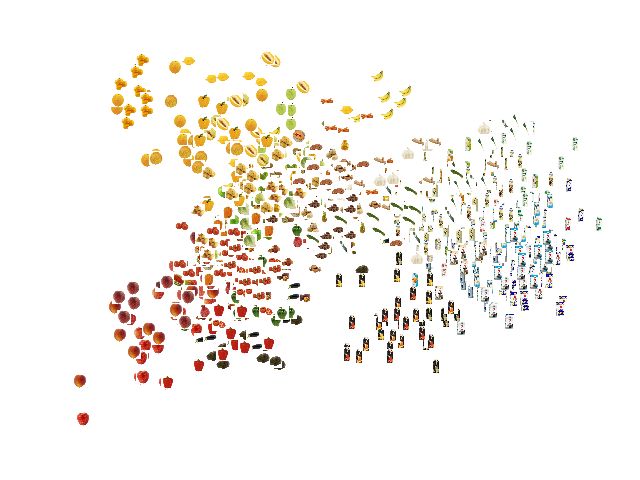
\includegraphics[width=\textwidth]{PaperB/appendix/figures/vcca_private_xi/pca_vcca_xi.png}
        	\caption{$\mu_{z}$ from VCCA$_{x i}$}
        	\label{fig:pca_vcca_xi_z}
        \end{subfigure}~
        \begin{subfigure}[t]{0.48\textwidth}
    		\centering
    		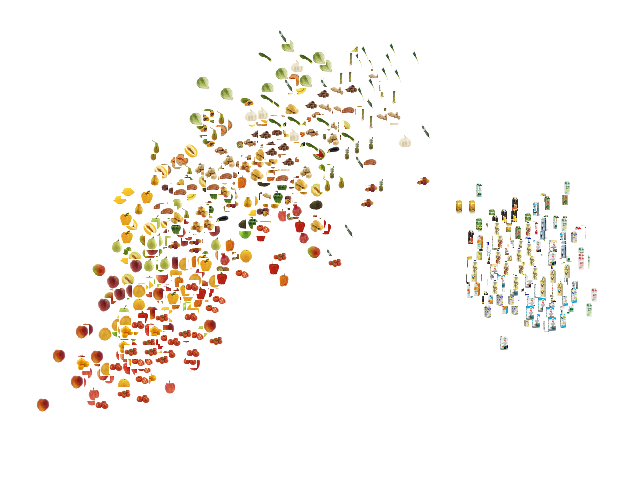
\includegraphics[width=\textwidth]{PaperB/appendix/figures/vcca_private_xi/pca_z_vcca_private_xi_seed1.png}
    		\caption{$\mu_{z}$ from VCCA-private$_{x i}$}
    		\label{fig:pca_vcca_private_xi_z}
    	\end{subfigure}
        %\subfigure[$\mu_{z}$ from VCCA$_{x i}$ ]{\label{fig:pca_vcca_xi_z}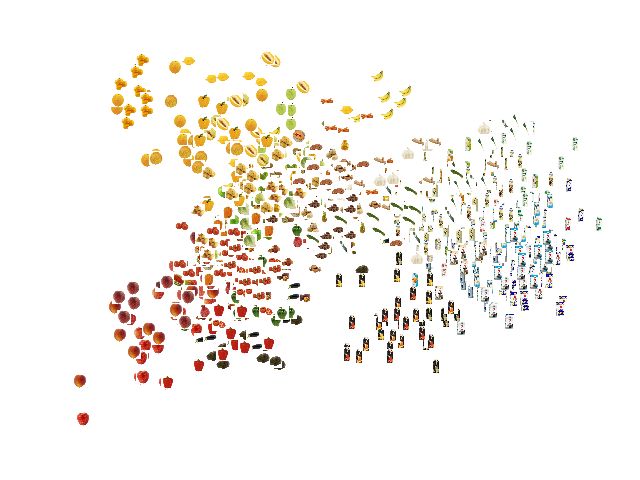
\includegraphics[width=0.45\textwidth]{PaperB/appendix/figures/vcca_private_xi/pca_vcca_xi.png}}~
        %\subfigure[$\mu_{z}$ from VCCA-private$_{x i}$]{\label{fig:pca_vcca_private_xi_z}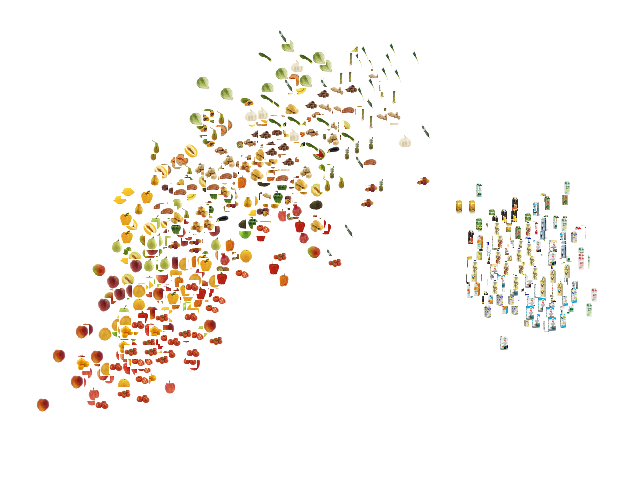
\includegraphics[width=0.45\textwidth]{PaperB/appendix/figures/vcca_private_xi/pca_z_vcca_private_xi_seed1.png}}\\ 
    \end{minipage}
    \begin{minipage}{0.8\textwidth}
        \centering
        \begin{subfigure}[t]{0.6\textwidth}
        	\centering
        	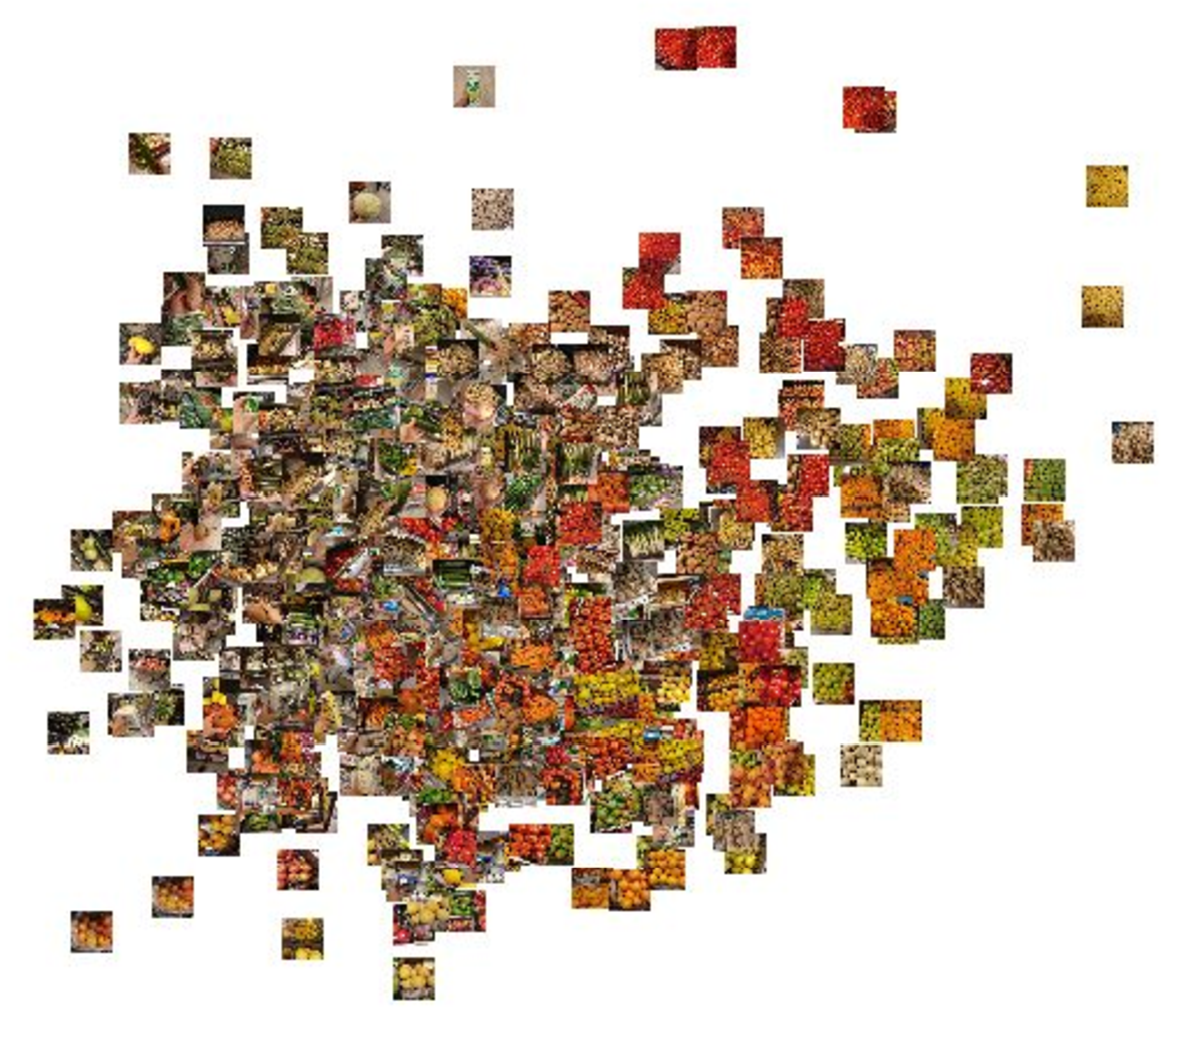
\includegraphics[width=\textwidth]{PaperB/appendix/figures/vcca_private_xi/vcca_private_xi_ux_space.pdf}
        	\caption{$\mu_{u_{x}}$ from VCCA-private$_{x i}$}
        	\label{fig:pca_vcca_private_xi_ux}
        \end{subfigure} \\
        \begin{subfigure}[t]{0.75\textwidth}
	    	\centering
	    	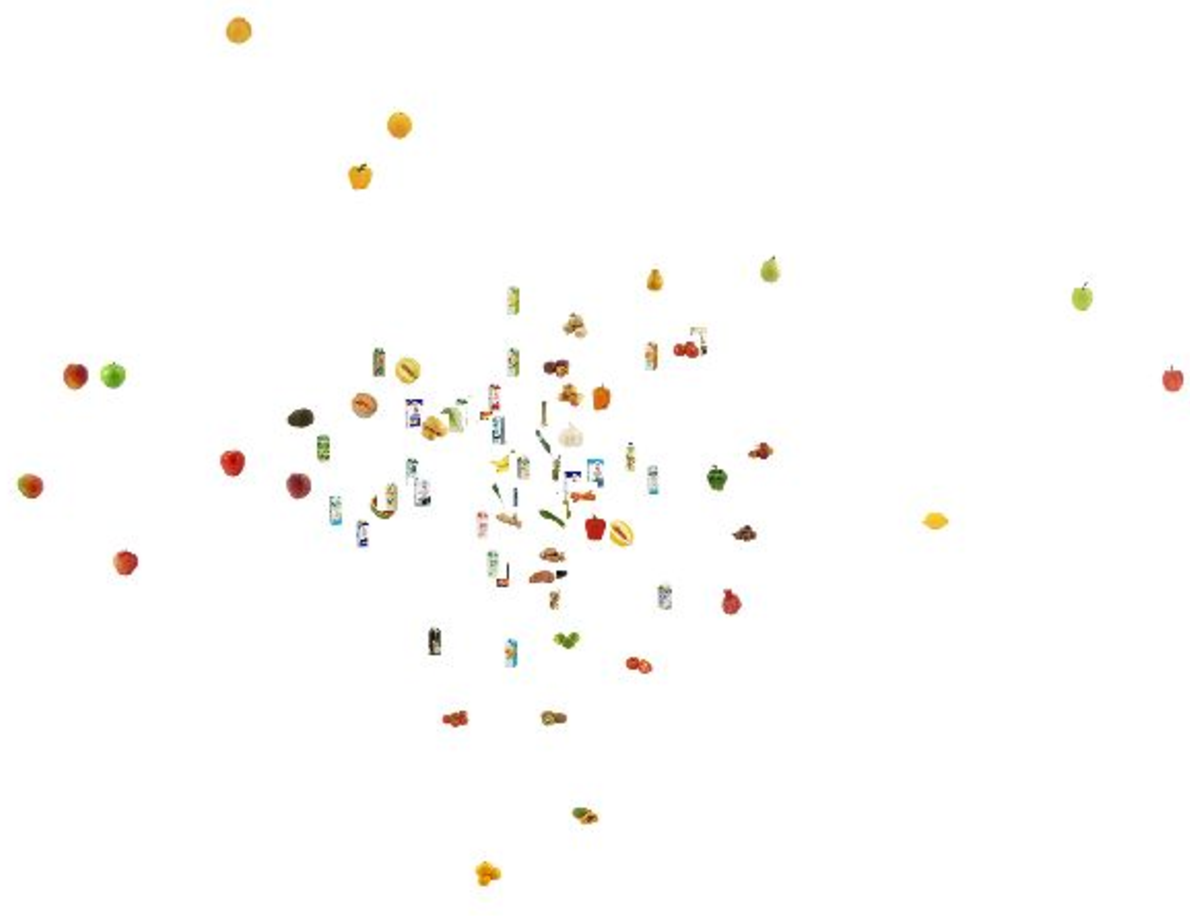
\includegraphics[width=\textwidth]{PaperB/appendix/figures/vcca_private_xi/vcca_private_xi_ui_space.pdf}
	    	\caption{$\mu_{u_{i}}$ from VCCA-private$_{x i}$}
	    	\label{fig:pca_vcca_private_xi_ui}
	    \end{subfigure}
    \end{minipage}
    \caption{Visualizations of the latent representations $\mu_{z}(x)$ from VCCA$_{x i}$ and VCCA-private$_{x i}$ on the first row followed by $\mu_{u_{x}}(x)$ and $\mu_{u_{i}}(i)$ for VCCA-private$_{x i}$. Abbreviations: VCCA, Variational Canonical Correlation Analysis.}
    \label{fig:2d_visualizations_pca_vcca_private_xi}
\end{figure}

\clearpage

%\resizebox{\textwidth}{!}{
\begin{figure}[t!]
    \centering
    %\resizebox{\textwidth}{!}{
    \begin{minipage}[t]{\textwidth}
        %\centering
        \begin{subfigure}[t]{0.21\textwidth}
        	\centering
        	% model_lda.tex
%
% Copyright (C) 2010,2011 Laura Dietz
% Copyright (C) 2012 Jaakko Luttinen
%
% The MIT License
%
% See LICENSE file for more details.

% Latent Diriclet allocation model
\tikzstyle{obs}=[circle,draw=black!50,fill=gray!25,thick,inner sep=0pt,minimum size=6mm]
\tikzstyle{latent}=[circle,draw=black!50,thick,inner sep=0pt,minimum size=6mm]
\tikzstyle{solid}=[draw=black!50, thick, >=stealth]

% Had to add ghost node because caption VAE_x didn't fit on one line...
\tikzstyle{ghost}=[circle,draw=white,thick,inner sep=0pt,minimum size=4mm]

\begin{tikzpicture}[x=1.cm,y=1.cm]

  % Nodes
  \node[obs]                    (x)    {$x$} ; %
  \node[ghost, right=0.1cm of x] (ghost1) {};
  \node[ghost, left=0.1cm of x] (ghost2) {};
  \node[latent, above=of x]    (z)     {$z$} ; %
  
  % Factors
  % Connect nodes
  \edge [solid] {z} {x} ; %

\end{tikzpicture}


        	%\includegraphics[width=\textwidth]{PaperB/appendix/figures/tikz_figures/vae_x}
        	\caption{VAE$_{x}$}
        	\label{fig:tikz_vae_x}
        \end{subfigure} \hspace{2mm}
    	\begin{subfigure}[t]{0.21\textwidth}
    		\centering
    		% model_lda.tex
%
% Copyright (C) 2010,2011 Laura Dietz
% Copyright (C) 2012 Jaakko Luttinen
%
% The MIT License
%
% See LICENSE file for more details.

% Latent Diriclet allocation model

\tikzstyle{obs}=[circle,draw=black!50,fill=gray!25,thick,inner sep=0pt,minimum size=6mm]
\tikzstyle{latent}=[circle,draw=black!50,thick,inner sep=0pt,minimum size=6mm]
\tikzstyle{solid}=[draw=black!50, thick, >=stealth]

\begin{tikzpicture}[x=1.cm,y=1.cm]

  % Nodes
  \node[obs]                    (x)    {$x$} ; %
  \node[obs, right=1.0cm of x]  (y)    {$y$} ; %
  \node[latent, above right=1.2cm and .4cm of x]    (z)     {$z$} ; %
  
  % Factors
  % Connect nodes
  \edge [solid] {z} {x} ; %
  \edge [solid] {z} {y} ; %

\end{tikzpicture}


    	%\includegraphics[width=\textwidth]{PaperB/appendix/figures/tikz_figures/vae_x}
    	\caption{VCCA$_{x y}$}
    	\label{fig:tikz_vcca_xy}
    	\end{subfigure} \hspace{2mm}
        \begin{subfigure}[t]{0.21\textwidth}
	    	\centering
	    	% model_lda.tex
%
% Copyright (C) 2010,2011 Laura Dietz
% Copyright (C) 2012 Jaakko Luttinen
%
% The MIT License
%
% See LICENSE file for more details.

% Latent Diriclet allocation model

\tikzstyle{obs}=[circle,draw=black!50,fill=gray!25,thick,inner sep=0pt,minimum size=6mm]
\tikzstyle{latent}=[circle,draw=black!50,thick,inner sep=0pt,minimum size=6mm]
\tikzstyle{solid}=[draw=black!50, thick, >=stealth]

\begin{tikzpicture}[x=1.cm,y=1.cm]

  % Nodes
  \node[obs]                    (x)    {$x$} ; %
  \node[obs, right=1.cm of x]  (i)    {$i$} ; %
  \node[latent, above right=1.2cm and .4cm of x]    (z)     {$z$} ; %
  
  % Factors
  % Connect nodes
  \edge [solid] {z} {x} ; %
  \edge [solid] {z} {i} ; %

\end{tikzpicture}


		    %\includegraphics[width=\textwidth]{PaperB/appendix/figures/tikz_figures/vae_x}
		    \caption{VCCA$_{x i}$}
		    \label{fig:tikz_vcca_xi}
		\end{subfigure} \hspace{2mm}
		\begin{subfigure}[t]{0.21\textwidth}
			\centering
			% model_lda.tex
%
% Copyright (C) 2010,2011 Laura Dietz
% Copyright (C) 2012 Jaakko Luttinen
%
% The MIT License
%
% See LICENSE file for more details.

% Latent Diriclet allocation model

\tikzstyle{obs}=[circle,draw=black!50,fill=gray!25,thick,inner sep=0pt,minimum size=6mm]
\tikzstyle{latent}=[circle,draw=black!50,thick,inner sep=0pt,minimum size=6mm]
\tikzstyle{solid}=[draw=black!50, thick, >=stealth]

\begin{tikzpicture}[x=1.cm,y=1.cm]

  % Nodes
  \node[obs]                    (x)    {$x$} ; %
  \node[obs, right=0.45cm of x]  (i)    {$i$} ; %
  \node[obs, right=0.45cm of i]  (y)    {$y$} ; %
  \node[latent, above= of i]    (z)     {$z$} ; %
  
  % Factors
  % Connect nodes
  \edge [solid] {z} {x} ; %
  \edge [solid] {z} {y} ; %
  \edge [solid] {z} {i} ; %

\end{tikzpicture}


			%\includegraphics[width=\textwidth]{PaperB/appendix/figures/tikz_figures/vae_x}
			\caption{VCCA$_{x i y}$}
			\label{fig:tikz_vcca_xiy}
		\end{subfigure} 
		\\[3mm]
        \begin{subfigure}[t]{0.20\textwidth}
         	\centering
         	% model_lda.tex
%
% Copyright (C) 2010,2011 Laura Dietz
% Copyright (C) 2012 Jaakko Luttinen
%
% The MIT License
%
% See LICENSE file for more details.

% Latent Diriclet allocation model

\tikzstyle{obs}=[circle,draw=black!50,fill=gray!25,thick,inner sep=0pt,minimum size=6mm]
\tikzstyle{latent}=[circle,draw=black!50,thick,inner sep=0pt,minimum size=6mm]
\tikzstyle{solid}=[draw=black!50, thick, >=stealth]

\begin{tikzpicture}[x=1.cm,y=1.cm]

  % Nodes
  \node[obs]                    (x)    {$x$} ; %
  \node[obs, right=1.cm of x]  (w)    {$w$} ; %
  \node[latent, above right=1.2cm and .4cm of x]    (z)     {$z$} ; %
  
  % Factors
  % Connect nodes
  \edge [solid] {z} {x} ; %
  \edge [solid] {z} {w} ; %

\end{tikzpicture}


         	\caption{VCCA$_{x w}$}
         	\label{fig:tikz_vcca_xw}
         \end{subfigure} \hspace{2mm}
         \begin{subfigure}[t]{0.20\textwidth}
         	\centering
         	% model_lda.tex
%
% Copyright (C) 2010,2011 Laura Dietz
% Copyright (C) 2012 Jaakko Luttinen
%
% The MIT License
%
% See LICENSE file for more details.

% Latent Diriclet allocation model

\tikzstyle{obs}=[circle,draw=black!50,fill=gray!25,thick,inner sep=0pt,minimum size=6mm]
\tikzstyle{latent}=[circle,draw=black!50,thick,inner sep=0pt,minimum size=6mm]
\tikzstyle{solid}=[draw=black!50, thick, >=stealth]

\begin{tikzpicture}[x=1.cm,y=1.cm]

  % Nodes
  \node[obs]                    (x)    {$x$} ; %
  \node[obs, right=0.45cm of x]  (w)    {$w$} ; %
  \node[obs, right=0.45cm of w]  (y)    {$y$} ; %
  \node[latent, above= of w]    (z)     {$z$} ; %
  
  % Factors
  % Connect nodes
  \edge [solid] {z} {x} ; %
  \edge [solid] {z} {y} ; %
  \edge [solid] {z} {w} ; %

\end{tikzpicture}


         	%\includegraphics[width=\textwidth]{PaperB/appendix/figures/tikz_figures/vae_x}
         	\caption{VCCA$_{x w y}$}
         	\label{fig:tikz_vcca_xwy}
         \end{subfigure} \hspace{2mm}
         \begin{subfigure}[t]{0.20\textwidth}
         	\centering
         	% model_lda.tex
%
% Copyright (C) 2010,2011 Laura Dietz
% Copyright (C) 2012 Jaakko Luttinen
%
% The MIT License
%
% See LICENSE file for more details.

% Latent Diriclet allocation model

\tikzstyle{obs}=[circle,draw=black!50,fill=gray!25,thick,inner sep=0pt,minimum size=6mm]
\tikzstyle{latent}=[circle,draw=black!50,thick,inner sep=0pt,minimum size=6mm]
\tikzstyle{solid}=[draw=black!50, thick, >=stealth]

\begin{tikzpicture}[x=1.cm,y=1.cm]

  % Nodes
  \node[obs]                    (x)    {$x$} ; %
  \node[obs, right=0.45cm of x]  (i)    {$i$} ; %
  \node[obs, right=0.45cm of i]  (w)    {$w$} ; %
  \node[latent, above= of i]    (z)     {$z$} ; %
  
  % Factors
  % Connect nodes
  \edge [solid] {z} {x} ; %
  \edge [solid] {z} {i} ; %
  \edge [solid] {z} {w} ; %

\end{tikzpicture}


         	%\includegraphics[width=\textwidth]{PaperB/appendix/figures/tikz_figures/vae_x}
         	\caption{VCCA$_{x i w}$}
         	\label{fig:tikz_vcca_xiw}
         \end{subfigure} \hspace{2mm}
         \begin{subfigure}[t]{0.20\textwidth}
         	\centering
         	% model_lda.tex
%
% Copyright (C) 2010,2011 Laura Dietz
% Copyright (C) 2012 Jaakko Luttinen
%
% The MIT License
%
% See LICENSE file for more details.

% Latent Diriclet allocation model

\tikzstyle{obs}=[circle,draw=black!50,fill=gray!25,thick,inner sep=0pt,minimum size=6mm]
\tikzstyle{latent}=[circle,draw=black!50,thick,inner sep=0pt,minimum size=6mm]
\tikzstyle{solid}=[draw=black!50, thick, >=stealth]

\begin{tikzpicture}[x=1.cm,y=1.cm]

  % Nodes
  \node[obs]                    (x)    {$x$} ; %
  \node[obs, right=0.3cm of x]  (i)    {$i$} ; %
  \node[obs, right=0.3cm of i]  (w)    {$w$} ; %
  \node[obs, right=0.3cm of w]  (y)    {$y$} ; %
  \node[latent, above right=1.2cm and .05cm of i]    (z)     {$z$} ; %
  
  % Factors
  % Connect nodes
  \edge [solid] {z} {x} ; %
  \edge [solid] {z} {i} ; %
  \edge [solid] {z} {w} ; %
  \edge [solid] {z} {y} ; %

\end{tikzpicture}


         	%\includegraphics[width=\textwidth]{PaperB/appendix/figures/tikz_figures/vae_x}
         	\caption{VCCA$_{x i w y}$}
         	\label{fig:tikz_vcca_xiwy}
         \end{subfigure}
     	\\[3mm]
     	\begin{subfigure}[t]{0.21\textwidth}
     		\centering
     		% model_lda.tex
%
% Copyright (C) 2010,2011 Laura Dietz
% Copyright (C) 2012 Jaakko Luttinen
%
% The MIT License
%
% See LICENSE file for more details.

% Latent Diriclet allocation model

\tikzstyle{obs}=[circle,draw=black!50,fill=gray!25,thick,inner sep=0pt,minimum size=6mm]
\tikzstyle{latent}=[circle,draw=black!50,thick,inner sep=0pt,minimum size=6mm]
\tikzstyle{solid}=[draw=black!50, thick, >=stealth]

\begin{tikzpicture}[x=1.cm,y=1.cm]

  % Nodes
  \node[obs]                    (x)    {$x$} ; %
  %\node[obs, right=0.45cm of x]  (y)    {$\vy$} ; %
  \node[obs, right=1.2cm of x]  (i)    {$i$} ; %
  \node[latent, above= of x]    (ux)     {$u_{x}$} ; %
  \node[latent, right=0.3cm of ux]    (z)     {$z$} ; %
  \node[latent, right= 0.3cm of z]    (ui)     {$u_{i}$} ; %
  
  % Factors
  % Connect nodes
  \edge [solid] {z} {x} ; %
  \edge [solid] {z} {i} ; %
  \edge [solid] {ux} {x} ; %
  \edge [solid] {ui} {i} ; %

\end{tikzpicture}


     		\caption{VCCA-private$_{x i}$}
     		\label{fig:tikz_vcca_private_xi}
     	\end{subfigure} \hspace{2mm}
     	\begin{subfigure}[t]{0.21\textwidth}
     		\centering
     		% model_lda.tex
%
% Copyright (C) 2010,2011 Laura Dietz
% Copyright (C) 2012 Jaakko Luttinen
%
% The MIT License
%
% See LICENSE file for more details.

% Latent Diriclet allocation model

\tikzstyle{obs}=[circle,draw=black!50,fill=gray!25,thick,inner sep=0pt,minimum size=6mm]
\tikzstyle{latent}=[circle,draw=black!50,thick,inner sep=0pt,minimum size=6mm]
\tikzstyle{solid}=[draw=black!50, thick, >=stealth]

\begin{tikzpicture}[x=1.cm,y=1.cm]

  % Nodes
  \node[obs]                    (x)    {$x$} ; %
  \node[obs, right=0.3cm of x]  (y)    {$y$} ; %
  \node[obs, right=0.3cm of y]  (i)    {$i$} ; %
  \node[latent, above= of x]    (ux)     {$u_{x}$} ; %
  \node[latent, above=of y]    (z)     {$z$} ; %
  \node[latent, above= of i]    (ui)     {$u_{i}$} ; %
  
  % Factors
  % Connect nodes
  \edge [solid] {z} {x} ; %
  \edge [solid] {z} {i} ; %
  \edge [solid] {z} {y} ; %
  \edge [solid] {ux} {x} ; %
  \edge [solid] {ui} {i} ; %

\end{tikzpicture}


     		%\includegraphics[width=\textwidth]{PaperB/appendix/figures/tikz_figures/vae_x}
     		\caption{VCCA-private$_{x i y}$}
     		\label{fig:tikz_vcca_private_xiy}
     	\end{subfigure} \hspace{2mm}
     	\begin{subfigure}[t]{0.21\textwidth}
     		\centering
     		% model_lda.tex
%
% Copyright (C) 2010,2011 Laura Dietz
% Copyright (C) 2012 Jaakko Luttinen
%
% The MIT License
%
% See LICENSE file for more details.

% Latent Diriclet allocation model

\tikzstyle{obs}=[circle,draw=black!50,fill=gray!25,thick,inner sep=0pt,minimum size=6mm]
\tikzstyle{latent}=[circle,draw=black!50,thick,inner sep=0pt,minimum size=6mm]
\tikzstyle{solid}=[draw=black!50, thick, >=stealth]

\begin{tikzpicture}[x=1.cm,y=1.cm]

  % Nodes
  \node[obs]                    (x)    {$x$} ; %
  %\node[obs, right=0.45cm of x]  (y)    {$y$} ; %
  \node[obs, right=1.2cm of x]  (w)    {$w$} ; %
  \node[latent, above= of x]    (ux)     {$u_{x}$} ; %
  \node[latent, right=0.3cm of ux]    (z)     {$z$} ; %
  \node[latent, right=0.3cm of z]    (uw)     {$u_{w}$} ; %
  
  % Factors
  % Connect nodes
  \edge [solid] {z} {x} ; %
  \edge [solid] {z} {w} ; %
  \edge [solid] {ux} {x} ; %
  \edge [solid] {uw} {w} ; %

\end{tikzpicture}


     		%\includegraphics[width=\textwidth]{PaperB/appendix/figures/tikz_figures/vae_x}
     		\caption{VCCA-private$_{x w}$}
     		\label{fig:tikz_vcca_private_xw}
     	\end{subfigure} \hspace{2mm}
     	\begin{subfigure}[t]{0.21\textwidth}
     		\centering
     		% model_lda.tex
%
% Copyright (C) 2010,2011 Laura Dietz
% Copyright (C) 2012 Jaakko Luttinen
%
% The MIT License
%
% See LICENSE file for more details.

% Latent Diriclet allocation model

\tikzstyle{obs}=[circle,draw=black!50,fill=gray!25,thick,inner sep=0pt,minimum size=6mm]
\tikzstyle{latent}=[circle,draw=black!50,thick,inner sep=0pt,minimum size=6mm]
\tikzstyle{solid}=[draw=black!50, thick, >=stealth]

\begin{tikzpicture}[x=1.cm,y=1.cm]

  % Nodes
  \node[obs]                    (x)    {$x$} ; %
  \node[obs, right=0.3cm of x]  (y)    {$y$} ; %
  \node[obs, right=0.3cm of y]  (w)    {$w$} ; %
  \node[latent, above= of x]    (ux)     {$u_{x}$} ; %
  \node[latent, above=of y]    (z)     {$z$} ; %
  \node[latent, above= of w]    (uw)     {$u_{w}$} ; %
  
  % Factors
  % Connect nodes
  \edge [solid] {z} {x} ; %
  \edge [solid] {z} {w} ; %
  \edge [solid] {z} {y} ; %
  \edge [solid] {ux} {x} ; %
  \edge [solid] {uw} {w} ; %

\end{tikzpicture}


     		%\includegraphics[width=\textwidth]{PaperB/appendix/figures/tikz_figures/vae_x}
     		\caption{VCCA-private$_{x w y}$}
     		\label{fig:tikz_vcca_private_xwy}
     	\end{subfigure}
    \end{minipage}
	%}
    \caption{ The graphical models of the VAE, VCCA, and VCCA-private, where nodes represent random variables and edges indicate possible dependence. Grey nodes are observed random variables, while white nodes are latent random variables. The joint distribution is given by the product of the conditional distributions of nodes given their parents. Abbreviations: VAE, Variational Autoencoder; VCCA, Variational Canonical Correlation Analysis.}
    \label{fig:graphical_models}
\end{figure}

\clearpage

\begin{table}[!ht]
    %\begin{adjustwidth}{-1cm}{}
    \centering
    \caption{Examples of text descriptions and their corresponding class label and iconic image from the Grocery Store dataset. }
    \vspace{-2mm}
    \resizebox{\textwidth}{!}{
    \begin{tabular}{c c c}
         \toprule
         {\bf\footnotesize Class Label} & {\bf\footnotesize Iconic Image} & {\bf\footnotesize Text Description} \\
         \toprule
         \multicolumn{1}{p{1.5cm}}{\vspace{-17mm} {\footnotesize Golden Delicious Apple} } &
          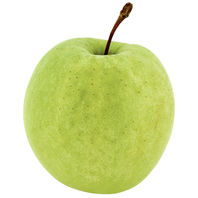
\includegraphics[width=21mm, height=21mm]{PaperB/appendix/figures/iconic_images/Golden-Delicious-Apple_Clean.jpg}  & 
         \multicolumn{1}{p{12cm}}{\vspace{-15mm} {\footnotesize Golden Delicious has a white juicy pulp and a greenish yellow shell. The taste is mellow and sweet, making Golden Delicious suitable for desserts.} } \\
         
         \toprule
         \multicolumn{1}{p{1.5cm}}{\vspace{-17mm} {\footnotesize Red Delicious Apple} } & 
          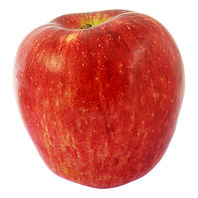
\includegraphics[width=21mm, height=21mm]{PaperB/appendix/figures/iconic_images/Red-Delicious-Apple_Clean.jpg}  &  
         \multicolumn{1}{p{12cm}}{\vspace{-15mm} {\footnotesize Red Delicious is a dark red apple with relatively soft pulp and sweet taste.} } \\
         
         \toprule
         \multicolumn{1}{p{1.5cm}}{\vspace{-15mm} {\footnotesize Orange} } & 
          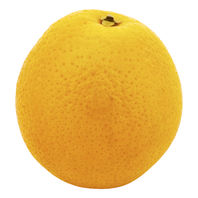
\includegraphics[width=21mm, height=21mm]{PaperB/appendix/figures/iconic_images/Orange_Clean.jpg}  & 
         \multicolumn{1}{p{12cm}}{\vspace{-17mm} {\footnotesize There are many different types of oranges that ripen and is sold during different parts of the year. The orange is a very important vitamin C source and the vitamins are best kept if the fruit is eaten naturally.} } \\
         
        \toprule
         \multicolumn{1}{p{1.5cm}}{\vspace{-15mm} {\footnotesize Yellow Bell Pepper} } & 
          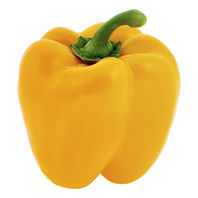
\includegraphics[width=21mm, height=21mm]{PaperB/appendix/figures/iconic_images/Yellow-Pepper_Clean.jpg}  &  
         \multicolumn{1}{p{12cm}}{\vspace{-19mm} {\footnotesize The yellow pepper is much sweeter than the green. It also contains more vitamins and antioxidants than the green. Peppers are good to eat raw in salads and as garnish, but are also good to fry, stew or gratinate, for example with filling. Paprika also fits well in pots, gratins and pies.} } \\
         
         \toprule
         \multicolumn{1}{p{1.5cm}}{\vspace{-15mm} {\footnotesize Orange Bell Pepper} } & 
          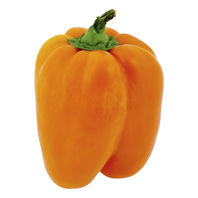
\includegraphics[width=21mm, height=21mm]{PaperB/appendix/figures/iconic_images/Orange-Bell-Pepper_Iconic.jpg}  & 
         \multicolumn{1}{p{12cm}}{\vspace{-17mm} {\footnotesize The orange pepper is sweeter than the green. It also contains more vitamins and antioxidants than the green. Peppers are good to eat raw in salads and as garnish, but are also good to fry, stew or gratinate, for example with filling. Paprika also fits well in pots, gratins and pies.} } \\
         
         \toprule
         \multicolumn{1}{p{1.5cm}}{\vspace{-17mm} {\footnotesize Arla Medium Fat Milk} } &
         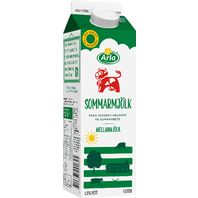
\includegraphics[width=21mm, height=21mm]{PaperB/appendix/figures/iconic_images/Arla-Milk-Medium-Fat_Clean.jpg} & 
         \multicolumn{1}{p{12cm}}{\vspace{-21mm} {\footnotesize Fresh skimmed milk made from Swedish milk from Arlagårdar. Skimmed milk has a delicious full-bodied milk flavor and is a popular choice for breakfast cereals, porridge or as a drink for the meal. Milk is a natural source of, for example, protein, calcium and vitamin B12. Protein contributes to muscle building and calcium is needed to maintain a normal bone structure. The brand Arla Ko guarantees that the product is made of 100\% Swedish milk.} } \\
         
         \toprule 
         \multicolumn{1}{p{1.5cm}}{\vspace{-18mm} {\footnotesize Arla Ecological Medium Fat Milk} } &
         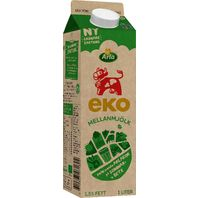
\includegraphics[width=21mm, height=21mm]{PaperB/appendix/figures/iconic_images/Arla-Ecological-Medium-Fat-Milk_Iconic.jpg} & 
         \multicolumn{1}{p{12cm}}{\vspace{-22mm} {\footnotesize Fresh skimmed milk made from Swedish milk from organic Arlagårdar. Skimmed milk has a delicious full flavor and is a popular choice for breakfast cereals, porridge or as a drink for the meal. Milk is a natural source of, for example, protein, calcium and vitamin B12. Protein contributes to muscle building and calcium is needed to maintain a normal bone structure. The brand Arla Ko guarantees that the product is made of 100\% Swedish milk. The new brown carton has 24 percent lower climate impact compared to the previous white carton.} } \\
         
         
        \toprule
         \multicolumn{1}{p{1.5cm}}{\vspace{-17mm} {\footnotesize God Morgon Orange Juice} } &
          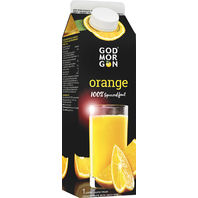
\includegraphics[width=21mm, height=21mm]{PaperB/appendix/figures/iconic_images/God-Morgon-Orange-Juice_Clean.jpg}  & 
         \multicolumn{1}{p{12cm}}{\vspace{-15mm} {\footnotesize God Morgon Orange is pressed by sun-dried, hand-picked oranges. The package contains juice from 2 kilograms of oranges!} } \\
         
         \toprule
         \multicolumn{1}{p{1.5cm}}{\vspace{-18mm} {\footnotesize Tropicana Golden Grapefruit Juice} } &
          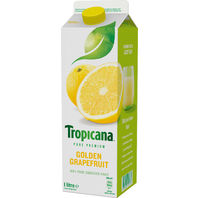
\includegraphics[width=21mm, height=21mm]{PaperB/appendix/figures/iconic_images/Tropicana-Golden-Grapefruit_Clean.jpg}  & 
         \multicolumn{1}{p{12cm}}{\vspace{-17mm} {\footnotesize Tropicana Golden Grape is a ready to drink juice with pulp pressed on grapefruit. Not from concentrate. Mildly pasteurized.} } \\
         
        \toprule
    \end{tabular}
	}

    \label{tab:grocerystore_dataset_descriptions}
    %\end{adjustwidth}
\end{table}

\clearpage

\begin{table}[h]
\centering
\caption{ Classification accuracies on the test set for all models in percentage (\%) along with the best hyperparameter setting, i.e., the scaling weights $\lambda$ and text description length $T$, for each model. The column Accuracy corresponds to the fine-grained classification accuracy. The column Coarse Accuracy corresponds to the classifying a class within the correct parent class. Results are averaged using 10 different random seeds and we report both means and standard deviations. Abbreviations: AE, Autoencoder; VAE, Variational Autoencoder; SplitAE, Split Autoencoder; VCCA, Variational Canonical Correlation Analysis.
}
\vspace{-2mm}
\resizebox{\textwidth}{!}{%\scalebox{0.95}{
\begin{tabular}{l | c c c c | c | c c}
    \hline
    \Xhline{3\arrayrulewidth}
    Model & $\lambda_{x}$ & $\lambda_{i}$ & $\lambda_{w}$ & $\lambda_{y}$ & $T$ & Accuracy (\%) & Coarse Accuracy (\%) \\
    \Xhline{3\arrayrulewidth} 
    {\small DenseNet-scratch} & - & - & - & - & - & $67.33 \pm 1.35$ & $75.67 \pm 1.15$ \\ \hline

    {\small Softmax} & - & - & - & - &  - & $71.67 \pm 0.28$ & $83.34 \pm 0.32$ \\ \Xhline{2\arrayrulewidth}
    {\small AE$_{x}$+Softmax} & 1 & - & - & - &  - & $70.69 \pm 0.82$ & $82.42 \pm 0.58$ \\ \hline
    {\small VAE$_{x}$+Softmax} & 1 & - & - & - &  - & $69.20 \pm 0.46$ & $81.24 \pm 0.63$ \\ \Xhline{2\arrayrulewidth}
    
    {\small SplitAE$_{x y}$} & 1 & - & - & 1000 &  - & $70.34 \pm 0.56$ & $82.11 \pm 0.38$ \\ \hline
    {\small VCCA$_{x y}$} & 1 & - & - & 1000 &  - & $70.72 \pm 0.56$ & $82.12 \pm 0.61$ \\ \Xhline{2\arrayrulewidth}
    
    {\small SplitAE$_{x i}$+Softmax} & 1 & 1000 & - & - & - & $77.68 \pm 0.69$ & $87.09 \pm 0.53$ \\ \hline 
    {\small VCCA$_{x i}$+Softmax} & 1 & 1000 & - & - &  - & $77.02 \pm 0.51$ & $86.46 \pm 0.42$ \\ \hline 
    {\small VCCA-private$_{x i}$+Softmax} & 1 & 10 & - & - &  - & $73.04 \pm 0.56$ & $84.16 \pm 0.51$ \\    
    \Xhline{2\arrayrulewidth}
    
    {\small SplitAE$_{x i y}$} & 1 & 1000 & - & 1000 &  - & $77.43 \pm 0.80$ & $87.14 \pm 0.57$ \\ \hline    
    {\small VCCA$_{x i y}$} & 1 & 1000 & - & 1000 &  - & $77.22 \pm 0.55$ & $86.54 \pm 0.51$ \\ \hline
    {\small VCCA-private$_{x i y}$} & 1 & 10 & - & 1000 &  - & $74.04 \pm 0.83$ & $84.59 \pm 0.83$ \\      
    \Xhline{2\arrayrulewidth}
    
    {\small SplitAE$_{x w}$+Softmax} & 1 & - & 1000 & - &  40 & $76.27 \pm 0.66$ & $86.45 \pm 0.56$ \\ \hline 
    {\small VCCA$_{x w}$+Softmax} & 1 & - & 1000 & - &  75 & $75.37 \pm 0.46$ & $86.00 \pm 0.32$ \\ \hline 
    {\small VCCA-private$_{x w}$+Softmax} & 1 & - & 1000 & - &  75 & $75.11 \pm 0.81$ & $85.91 \pm 0.55$ \\
    \Xhline{2\arrayrulewidth} 
    
    {\small SplitAE$_{x w y}$} & 1 & - & 1000 & 10 &  75 & $75.78 \pm 0.84$ & $86.13 \pm 0.63$ \\ \hline
    {\small VCCA$_{x w y}$} & 1 & - & 1000 & 10 &  75 & $74.72 \pm 0.85$ & $85.59 \pm 0.78$ \\ \hline
    {\small VCCA-private$_{x w y}$} & 1 & - & 1000 & 1000 & 50 & $74.92 \pm 0.74$ & $85.59 \pm 0.67$ \\       
    \Xhline{2\arrayrulewidth} 
    
    {\small SplitAE$_{x i w}$+Softmax} & 1 & 1000 & 1000 & - &  24 & $77.79 \pm 0.48$ & $87.12 \pm 0.62$ \\
    {\small VCCA$_{x i w}$+Softmax} & 1 & 1000 & 1000 & - &  32 & $77.51 \pm \, 0.51$ & $86.69 \pm 0.41$ \\ \Xhline{2\arrayrulewidth}   
    
    {\small SplitAE$_{x i w y}$} & 1 & 1000 & 1000 & 1000 & 24 & $78.18 \pm 0.53$ & $87.26 \pm 0.46$ \\ 
    {\small VCCA$_{x i w y}$} & 1 & 1000 & 1000 & 1000 &  91 & $77.78 \pm 0.45$ & $86.88 \pm 0.47$ \\ 
    \Xhline{3\arrayrulewidth}
\end{tabular}
}
\vspace{-2mm}
\label{tab:classification_results_on_test_set_with_hyperparameters}
\end{table}

%\clearpage

